% -*- root: ../Thesis.tex -*-
\chapter{Podstawy nieprzestrzennego modelowania dynamiki wapnia}
\label{chap:modelowanie:osc}


\section{Modelowanie przepływów przez pompy}

Pompy wapniowe działają podobnie jak enzymy, hydrolizując ATP wykonują pracę użyteczną komórce - mianowicie przenoszą określone cząsteczki w poprzek błony komórko-wej. Podobnie jak enzymy, pompy podlegają wielopoziomowej kontroli z miejscami inhibitorowymi i aktywatorowymi, które tworzą skomplikowaną sieć sprzężeń zwrotnych dodatnich i ujemnych. Podobnie jak w przypadku reakcji enzymatycznych, transport z udziałem pompy wapniowej odbiega od prawa działania mas. Dokładniej, prędkość przepływu jonów wapnia $V$ w poprzek błony biologicznej opisuje się najczęściej wzorem Michaelisa-Menten:


\begin{equation}
V = V_{max} \cdot \frac{[Ca^{2+}]}{K_m + [Ca^{2+}]}
\label{eq:Vc}
\end{equation}

\noindent gdzie $[Ca^{2+}]$ jest stężeniem jonów wapnia w odpowiednim kompartmencie, a $K_m$ stałą charakteryzującą pompę, nazywaną również stałą Michaelisa.

\bigskip

\noindent \textbf{\textit{Przypadek 1:}} $[Ca^{2+}] \ll K_m$\\
\noindent Jeżeli jony wapnia występują w niewielkim stężeniu, dużo mniejszym od $K_m$, to tempo transportu wapnia opisane wzorem (\ref{eq:Vc}) jest w przybliżeniu liniowo proporcjonalne do $[Ca^{2+}]$. Dokładniej:

\begin{equation}
V \sim \frac{V_{max} \cdot [Ca^{2+}]}{K_m} = k \cdot [Ca^{2+}]
\end{equation}

\noindent gdzie $k=\frac{V_{max}}{K_m}$.
\bigskip


\noindent \textbf{\textit{Przypadek 2:}} $[Ca^{2+}] = K_m$\\

Gdy stężenie substratu równe jest stałej Michelisa, prędkość przepływu wynosi dokładnie połowę prędkości maksymalnej:

\begin{equation}
V = \frac{V_{max} \cdot [Ca^{2+}]}{[Ca^{2+}] + [Ca^{2+}]} = \frac{V_{max} \cdot [Ca^{2+}]}{2\cdot [Ca^{2+}]} = \frac{V_{max}}{2}
\end{equation}

Zależność tę wykorzystuje się do wyznaczania stałej $K_m$, która jest również miarą powinowactwa białka transportującego do wapnia - im mniejsza, tym powinowactwo jest większe, natomiast duża wartość tej stałej mówi o małym powinowactwie.

\bigskip

\noindent \textbf{\textit{Przypadek 3:}} $[Ca^{2+}] \gg K_m$\\

\begin{equation}
V \sim \frac{V_{max} \cdot [Ca^{2+}]}{[Ca^{2+}]} = V_{max}
\end{equation}


\section{Modelowanie przepływów przez kanały i~wymienniki}\label{s:hill}

Modelowanie transportu przez kanały i wymienniki również odbiega od klasycznej kinetyki Michaelisa-Menten stosowanej do opisu dynamiki reakcji enzymatycznych. Modelowanie tych przepływów oparte jest na funkcji Hilla, która bierze pod uwagę możliwość wiązania cząsteczek substratu (wapnia) i cząsteczek regulatorowych (regulacja allosteryczna) i opisuje pośrednio oddziaływanie pomiędzy nimi \cite{Keener2009,Harper2006}.
Funkcja ta ma następującą postać:

\begin{equation}
H(x) =  V_{max}\frac{x^n}{K_d^n+x^n}, \quad n>0
\label{eq:Hill}
\end{equation}

\noindent gdzie stała $n$ nazywana jest współczynnikiem Hilla i może być dowolną liczbą rzeczywistą, natomiast współczynniki V$_{max}$ i K$_d$ określają odpowiednio: wartość maksymalną i stałą pół-aktywacji. Mimo, iż wykładnik funkcji Hilla może przyjąć dowolną wartość, jest on z reguły wyznaczany empirycznie, a jego wartość zależy od ilości miejsc wiążących substrat/ligand oraz typu interakcji między nimi. Dla $n=1$ miejsca wiązania substratu i ligandu działają niezależnie, jeżeli $n>1$ miejsca są ,,kooperatywne'', to znaczy, że związanie ligandu w powoduje zwiększenie prawdopodobieństwa przyłączenia się substratu w pozostałych. W ten sposób funkcja Hilla specyficznie opisuje reakcje biologiczne oparte na mechanizmie ON/OFF. Wykładnik Hilla decyduje o tym jaki kształt przyjmie krzywa. Im większe $n$ (i dostatecznie duże), tym szybsze zmiany w~punkcie
$x_p= K_d \left(\frac{n-1}{n+1}\right)^{1/n}$ przegięcia funkcji, w którym pochodna przyjmuje wartość maksymalną. Z tego względu funkcja Hilla o dużym $n$ nazywana jest również funkcją przełączeniową \cite{Gunter1990}. Uwagi odnoszące się do Przypadków 1-3 poprzedniego podrozdziału pozostają w mocy również dla funkcji Hilla opisanej wzorem~(\ref{eq:Hill}).

Prostymi przykładami kanałów związanych z transportem wapnia, często opisywanych funkcją Hilla
(\ref{eq:Hill}) są receptory: rianodynowy (RyR) i receptor IP$_3$ (IP$_3$R), znajdujące się w błonach siateczki sródplazmatycznej.

Bardziej skomplikowanymi kanałami wapniowymi są transportery przenoszące jednocześnie dwa substraty. Przykładem takiego białka jest wymiennik sodowo-wapniowy (NCX), znajdujący się na  wewnętrznej błonie mitochondrialnej. Białko to przenosi jon wapnia do przestrzeni międzybłonowej i trzy jony sodu do wnętrza mitochondrium. Transport tego typu modelowany jest poprzez iloczyn dwóch funkcji Hilla:

\begin{equation} \label{eq:NCAfluxes}
J_{NCX} = V_{NCX} \frac{Ca_{Cyt}^{n}}{K_{Ca}^{n} + Ca_{Cyt}^{n}}\;\;\frac{Na_{Cyt}}{K_{Na} + Na_{Cyt}}
\end{equation}

\noindent gdzie $Ca_{Cyt}$ to stężenie wolnego wapnia w cytozolu, $K_{Ca}$ określa stałą pół-aktywacji dla jonów wapnia, natomiast K$_{Na}$ określa stałą pół-aktywacji dla jonów sodu.

\bigskip

\noindent \textbf{Uwaga:}
We wzorze (\ref{eq:NCAfluxes}) oznaczenie stężenia jonów wapnia w cytozolu  $[Ca^{2+}]_{Cyt}$  zostało uproszczone do $Ca_{Cyt}$. Podobna konwencja stosowana będzie również w dalszym ciągu pracy do stężenia jonów wapnia w pozostałych kompartmentach, to znaczy $[Ca^{2+}]_{Mit}$ będzie oznaczane symbolem $Ca_{Mit}$, natomiast $[Ca^{2+}]_{ER}$ symbolem $Ca_{ER}$.

\bigskip

Modelowanie uniportera jest jeszcze bardziej złożone, ponieważ istotną rolę w jego funkcji odgrywa potencjał transbłonowy $\Delta\Psi_m$, wprowadzony w Rozdz.~\ref{ss:uniporter}.

\noindent Już w 1990 roku Gunter i Pfeifer \cite{Gunter1990} wykorzystali równanie Nernsta  do odtworzenia potencjału błonowego w mitochondriach, który jest siłą napędową działania MICU. Pobieranie wapnia przez mitochondria z uwzględnieniem  $\Delta\Psi_m$ opisuje się równaniem:

\begin{equation}
J_{uni}=V_{uni} \frac{ZF\Delta\psi}{RT}\;e^{ZF\Delta\psi/RT}\;\;sinh\left(\frac{ZF\Delta\psi}{RT}\right)\;\frac{Ca_{cyt}^2}{K^{2}_{Ca} + Ca_{cyt}^2}
\end{equation}

\noindent (por. formuła (33) w \cite{Falcke2004}), gdzie $\Delta\psi$ jest efektywnym potencjałem transbłonowym, $R$ - stałą gazową, $Z$ stechiometria ładunków, $F$ - stałą Faradaya, natomiast $T$ to temperatura mierzona w skali Kelvina.
Efektywny potencjał transbłonowy określa się poprzez
potencjał transbłonowy $\Delta\Psi_m$
za pomocą równania:

\[  \Delta\psi = b (\Delta\Psi_m - \Delta\Psi_{m0}) \]

\noindent gdzie $\Delta\Psi_{m0}$ oraz $b$ są parametrami empirycznymi. Parametry te
odzwierciedlają fakt, że potencjał $\Delta\Psi_m$ nie jest stały wzdłuż błony
mitichondrialnej.

%\noindent Takie podejście wydaje się być bardzo efektywne i dodaje do każdego modelu podstawową dynamikę poboru i uwalniania wapnia z mitochondriów. Jednakże tego typu uproszczenia pomijają bardzo istotny aspekt, jakim jest potencjał transbłonowy  $\Delta\psi_m$. Mimo to powstały modele, które pomimo uproszczeń są w stanie symulować wewnątrzkomórkową dynamikę wapnia, która pozwala na badanie takich mechanizmów jak powstawanie złożonych oscylacji wapniowych (np. \cite{Marhl2000}), uwalnianie pęcherzyków komórek wydzielniczych trzustki \cite{Sneyd2003} lub zwiększonego poboru jonów Ca$^{2+}$ przez naergetyzowane mitochondria \cite{Thul2008}.

Równocześnie Magnus i Keizer stworzyli całościowy model aktywności elektrycznej mitochondriów \cite{Magnus1998}. Model ten zadany jest przez równania różniczkowe zwyczajne opisujące m.in. ewolucję czasową $J_{H,res}$ (wypływ H$^+$ indukowany przez łańcuch oddechowy); $J_{H,F1}$ (napływ jonów H$^+$ poprzez syntezę ATP); $J_{ant}$ (wymiennik nukleotydów adeninowych - Adenin Nucleotide Translocator - wymieniający ATP na ADP), $J_{uni}$ (przepływ jonów wapnia do macierzy w wyniku działania uniportera mitochondrialnego)
oraz efektywny potencjał transbłonowy $\Delta \psi$ \cite{Falcke2004} zmieniający się zgodnie z~równaniem:

\begin{equation}
C_{mit}\frac{d\Delta\psi}{dt}=-\left(-J_{H,res}+J_{H,F1}+J_{ant}+J_{H_leak}+2J_{uni}\right)
\end{equation}


\noindent Przepływ przez uniporter mitochondrialny $J_{uni}$ w powyższej pracy ma postać:

\begin{equation}
{ J }_{ uni }={ V }_{ uni }\frac { \frac { { Ca }_{ cyt } }{ { K }_{ trans } } { \left( 1+\frac { { Ca }_{ cyt } }{ { K }_{ trans } }  \right)  }^{ 3 } }{ { \left( 1+\frac { { Ca }_{ cyt } }{ { K }_{ trans } }  \right)  }^{ 4 }\quad +\quad \frac { L }{ { \left( 1+\frac { { Ca }_{ cyt } }{ { K }_{ act } }  \right)  }^{ { n }_{ a } } }  } \quad \frac { \frac { \left( ZF\left( \Delta \phi -91mV \right)  \right)  }{ RT }  }{ 1-{ e }^{ -{ \left( ZF\left( \Delta \phi -91mV \right)  \right)  }/{ \left( RT \right)  } } }
\end{equation}

\noindent gdzie $Ca_{cyt}$ określa stężenie wolnych jonów wapnia w cytozolu, $n=2.8$, natomiast stałe $K_{trans}$ i $K_{act}$ to stałe dysocjacji jonów wapnia dla miejsca transportującego i~miejsca aktywującego. Przedstawione powyżej modele były bardzo pomocne w pomiarach maksymalnej prędkości transportu jonów wapnia do mitochondrium, oznaczanej jako V$_{uni}$.



Wypływ wapnia z mitochondrium poprzez wymiennik mNCX (Rozdz.~\ref{ch:NCX}) opisane zostało w~pracy \cite{Magnus1998} wyrażeniem:

\begin{equation}
{ J }_{NCX}={ V }_{ NCX }\quad \frac { { e }^{ \left( { bF\left( \Delta \phi -91\, mV \right)  }/{ RT } \right)  } }{ { \left( 1+\frac { { K }_{ Na } }{ [Na] }  \right)  }^{ n }\left( 1+\frac { { K }_{ Ca } }{ Ca_{Mit} }  \right)  }
\end{equation}

\noindent gdzie $V_{NCX}$ to maksymalna prędkość transportu jonów wapnia, Ca$_{Mit}$ to stężenie wolnych jonów wapnia w mitochondrium. Stałe $n$ i $b$ określają charakter wymiany jonów $Na^+$ na jony $Ca^{2+}$. Tak więc $n=2$ i $b=0$, jeżeli wymieniane są 2 jony sodu na jeden jon wapnia, to znaczy, że jest ona neutralna elektrycznie. Jeśli natomiast trzy jony $Na^+$ wymieniane są na jeden jon $Ca^{2+}$ ($n=3$) i $b>0$. Z pracy \cite{Pradhan2010} wynika, że proporcje wymiany jonów dla mNCX to 3:1 dla par jonów sód:wapń \cite{Pradhan2010}.


\section{Szczegółowy model uniportera mitochondrialnego}

Innym interesującym zjawiskiem, badanym \emph{in silico} był tzw. mechanizm RaM (ang. calcium rapid uptake mode), który został zaproponowany w pracy \cite{Sparagna1995} w roku 1995. Praca ta sugeruje, że w warunkach ekspozycji na stężenie mniejsze niż 0.5-0.8 $\mu$M wapnia aktywny jest tzw. szybki mechanizm pobierania jonów wapniowych RaM. W tych warunkach mitochondria pobierają wapń znacznie wydajniej, jednak przez stosunkowo krótki okres czasu. Przepływ do mitochondriów składa się zatem z dwóch części. Pierwsza z nich uwzględnia wspomniany powyżej szybki mod RaMowy, druga opisuje prace uniportera mitochondrialnego w~trybie standardowym. Istnienie szybkiego mechanizmu  typu RaM zostało potwierdzone dzięki badaniom Buntinasa i~współpracowników, którzy badali mitochondria wyizolowane z kardiomiocytów szczura. W~eksperymentach tych mechanizm RaM został zidentyfikowany jako różny od regularnej działalności uniportera. Zachodzi na początku pulsu wapniowego i wyłącza się gdy stężenie wapnia na zewnątrz mitochondriów przekracza pewną wartość progową (co do rzędu wielkości równą 0.5-0.8$\mu$M). W obu rodzajach mitochondriów (wyizolowanych z hepatocytów i kardiomiocytów) dezaktywacja RaM zachodziła w~czasie krótszym niż 0.75 s \cite{Buntinas2001}. Przez ponad dekadę RaM postrzegany był jako nowy mechanizm  poboru wapnia przez mitochondria, nie związany z białkiem uniportera mitochondrialnego. Dopiero badania przeprowadzone przez Guntera i współpracowników wykazały, że może on mieć związek z tym uniporterem i stanowi dodatkowy sposób transportu jonów wapnia przez to białko \cite{Gunter2004}.


Matematyczny model mechanizmu RaM zaproponowali Dash i Basil \cite{Bazil2011,Dash2009}. Założyli oni, że uniporter może znajdować się w 5 różnych dyskretnych stanach, które opisują zmiany zachodzące w białku uniportera o związaniu jonów wapnia. Te stany to: R, O, I$_1$ oraz I$_2$ i dodatkowo S, którym odpowiadają kolejno następujące stany mitochondrialnego uniportera: stan spoczynkowy (\textbf{r}esting), otwarty (\textbf{o}pen), stany obniżonej aktywności 1 i 2 (\textbf{i}nhibited 1,2), powolny powrót do stanu wyjściowego (\textbf{S} - slow recovery state). Eksperymenty numeryczne Basil i Dash przeprowadzali na zredukowanym modelu, który obejmował dwa różne stany: R-O oraz I$_1$I$_2$, które odpowiadały stanom: spoczynkowo - otwartym i sumie stanów o obniżonej aktywności. Podczas symulacji stwierdzono, że podczas cyklu pobierania wapnia około 1/4 białek bardzo szybko przechodziło ze stanu RaM do stanu spoczynkowego, dla pozostałych uniporterów przejście zajmowało około 90 s. Dane te interpretowano jako przejście większości uniporterów w~stan wolnego pobierania jonów wapnia.

Stosunek białek znajdujących się w~stanie spoczynkowym, do białek znajdujących się w~stanie otwartym opisywało wyrażenie:


\begin{equation}
{ f }_{ Ca }=\frac { { \left[ { Ca }^{ 2+ } \right]  }^{ n } }{ { \left[ { Ca }^{ 2+ } \right]  }^{ n }+{ { K }_{0} }^{ n } }
\end{equation}

\noindent Stosunek pomiędzy pierwszym i drugim stanem $I$ wyliczana jest podobnie:

\begin{equation}
{ g }_{ Ca }=\frac { { \left[ { Ca }^{ 2+ } \right]  }^{ n } }{ { \left[ { Ca }^{ 2+ } \right]  }^{ n }+{ { K }_{ 1 } }^{ n } }
\end{equation}

\noindent Tempo wymiany jonów wapniowych poprzez RaM dane jest następującym wyrażeniem:

\begin{equation}
{ J }_{ RaM }={ X }_{ RaM }O\frac { { e }^{ { z }_{ Ca }\Delta \psi F/2RT }\left[ { Ca }^{ 2+ } \right] /{ K }_{ Ca } }{ 1+\left[ { Ca }^{ 2+ } \right] /{ K }_{ Ca } }
\end{equation}

\noindent W powyższych równaniach $n$ jest współczynnikiem funkcji Hilla charakteryzujący dynamikę wymiany; [Ca$^{2+}$]  oznacza stężenie wolnych jonów wapnia; $K_0$ - stężenie progowe wapnia, które jest w stanie uruchomić mechanizm wymiany; $K_1$ - stężenie progowe stabilizujące mechanizm wymiany w stanie inhibitorowym, $K_{Ca}$ - powinowactwo kompleksu RaM do jonów Ca$^{2+}$; $X_{RaM}$ aktywność RaM.

%Aby zredukować złożoność modelu autorzy założyli, że stan spoczynkowy i otwarty  ilość  parametrów, użyte zostało następujące uproszczenie modelu:
%
%
%\begin{equation}
%\frac { d{ \left[ { Ca }^{ 2+ } \right]  }_{ x } }{ dt } =\left( { J }_{ RaM }-{ J }_{ KCHE }\left( { \left[ { Ca }^{ 2+ } \right]  }_{ x }-{ \left[ { Ca }^{ 2+ } \right]  }_{ x,min } \right) +{ J }_{ CU } \right) /{ \beta  }_{ Ca }
%\end{equation}
%
%$J_{Ram}$; $J_{KCHE}$; $J_{CU}$;

Wykorzystując dane uzyskane z eksperymentów, Basil and Dash byli w stanie odtworzyć główne cechy transportu RaM. Symulacje wierne odtwarzały profile poboru jonów Ca$^{2+}$ dla stymulacji ciągłych i odtwarzały wzrost efektywności poboru w przypadku zastosowania wielokrotnych stymulacji w stosunku do pojedynczego, przedłużonego pulsu.

\section{Bufory wapniowe}\label{ch:bufory}

Około 99 \% jonów wapnia w komórce związana jest z białkami buforowymi (Tab.~\ref{tab:cabp}) lub buforami nieorganicznymi (cytryniany, fosforany). Do buforów cytoplazmatycznych należą m.in. kalbindyna, kalretynina i parvalbumina, w retikulum endoplazmatycznym do białek buforujących nalezą np. kalsekwestryna i kalretikulina. Stężenie białek buforowych jest głównym, ale nie jedynym czynnikiem kształtującym zdolność buforowania wapnia w komórce. Do innych równie istotnych należą kinetyka wiązania i dysocjacji Ca$^{2+}$, czy też mobilność samych buforów.

Reakcja chemiczna wiązania jonów wapnia przez bufor białkowy $Pr$:

\begin{equation}
\ce{Pr + Ca^{2+} <=>[k_+][k_-] PrCa}
\end{equation}

\noindent gdzie $Pr$ to białka buforujące, natomiast $PrCa$ oznacza zbuforowany wapń.

Odpowiadająca reakcji stała dysocjacji zdefiniowana jest poprzez równanie

\begin{equation}
K_d = \frac{[Pr]\cdot[Ca^{2+}]}{[PrCa]}
\end{equation}

\noindent w którym [$Pr$],[$Ca^{2+}$],[$PrCa$] oznaczają stężenia molowe odpowiednio białek buforujących, wolnych jonów wapnia i jony wapnia związane przez bufory.

Powyższa reakcja pozwala na utworzenie prostego modelu buforowania wapnia. Czasoprzestrzenne zmiany stężenia wolnych jonów wapnia w cytozolu, przy uwzględnieniu zjawisk buforowania opisuje się często w sposób przybliżony za pomocą następującego układu równań typu reakcji-dyfuzji:

\begin{footnotesize}
\begin{eqnarray}
\frac{\partial{Ca_{Cyt}}}{\partial{t}} &=& f(c) + \sum (k_{i-}Pr_iCa-k_{i+}Ca_{Cyt} (Pr_{i\, tot}-Pr_iCa))\\[.3em]
\frac{\partial{Pr_iCa}}{\partial{t}} &=& - \sum (k_{i-}Pr_iCa + k_{i+}Ca_{Cyt} (Pr_{i\, tot}-Pr_iCa))\\[.3em]
Pr_{i\, tot} &=& Pr_i + Pr_iCa
\end{eqnarray}
\end{footnotesize}

\noindent w którym $Pr_iCa$  oznacza stężenie buforu z przyłączonymi jonami wapnia, $Ca_{Cyt}$ wolne jony wapnia w cytozolu, $f(c)$ to wszystkie reakcje, które określają przepływy jonów wapnia (np. uwolnienie jonów poprzez receptory IP$_3$R, transport przez pompy wapniowe i~inne). $Pr_{tot}$ oznacza całkowite stężenie buforów.
\noindent Wielkości:

\begin{equation}
K_{di}: = \frac{[k_i+]}{k_{i-}}
\end{equation}

\noindent nazywane są  stałymi równowagi reakcji buforowania lub też stałymi dysocjacji. Wartości stałych dysocjacji dla niektórych buforów podano w Tab.~\ref{tab:cabp}.

\subsection{Modelowanie kompleksów błonowych}

Kompleksy błonowe zyskały na znaczeniu w ciągu ostatniej dekady, kiedy możliwe było wykorzystanie nowo-otrzymanych wskaźników jonów wapnia w postaci białek transgenicznych \cite{Alvarez2002,Brini1993,Cobbold1983,DelaFuente2013,Jung2004,Webb2012}. Metody te  pozwoliły na pomiar stężeń jonów wapnia w stosunkowo niewielkich przestrzeniach ograniczonych kompleksami błonowymi. Powstały specjalne konstrukty sensorów aequorynowych i białek strukturalnych wschodzących w skład danego kompleksu błonowego, które pozwoliły na oszacowanie zjawiska.

Niewielka ilość danych  eksperymentalnych na temat mechanizmu powstawania kompleksów błonowych i ich roli w procesach fizjologicznych komórki spowodowały, że jest to temat mało popularny dla naukowców związanych z biologią obliczeniową. Jedyny model, który dotyczył aspektu bliskiej apozycji różnego rodzaju struktur komórkowych w kontekście sygnalizacji wapniowej był model trój-kompartmentowy Marhla \cite{Marhl2000}.  Inne podejście zaprezentował Mazel \cite{Mazel2009}, który stworzył stochastyczny model  przestrzenny w geometrii trójwymiarowej, uzyskanej ze zdjęć komórek RBL-2H3 wykonanych mikrosko-pem konfokalnym. Mazel zwrócił szczególną uwagę na odległości pomiędzy poszczególnymi strukturami komórkowymi, jednak w przedstawionym przez niego modelu nie uzyskano oscylacji stężenia jonów wapnia.


\section{Oscylacje wapniowe}

Zmiany stężenia jonów wapnia w poszczególnych kompartmentach komórki, występują w~sposób naturalny w wielu rodzajach komórek. Pojawiają się spontanicznie w kardiomiocytach, hepatocytach, komórkach wydzielniczych trzustki lub neuronach. Oscylacje wapniowe pojawiają się również w odpowiedzi na różnego rodzaju bodźce, np. oscylacje w komórkach nabłonka płaskiego wyściełającego (komórkach endotelialnych), w odpowiedzi na infekcję bakteryjną lub  zmiany stężenia Ca$^{2+}$ w komórkach czuciowych skóry (w ciałkach Pacciniego oraz w ciałkach Ruffiniego) w odpowiedzi na bodziec mechaniczny \cite{Maeda1999, Vega1996}.

Zastosowanie metod pozwalających badanie zmian stężenia wapnia w pojedynczych komórkach lub nawet kompartmentach, pozwoliło odkryć różnego rodzaju oscylacje wapniowe o bardzo złożonym charakterze. W zależności od komórki okres tych oscylacji może wynosić od 1 sekundy do 10 minut. Przebiegi czasowe tych oscylacji mogą przyjmować różne kształty od ostrych pików z gwałtownym wzrostem (,,bursting"), do łagodnych o prawie  sinusoidalnym przebiegu, z dużą gamą form pośrednich Ryc.~\ref{fig:oscylacje}.

\begin{figure}
\centering
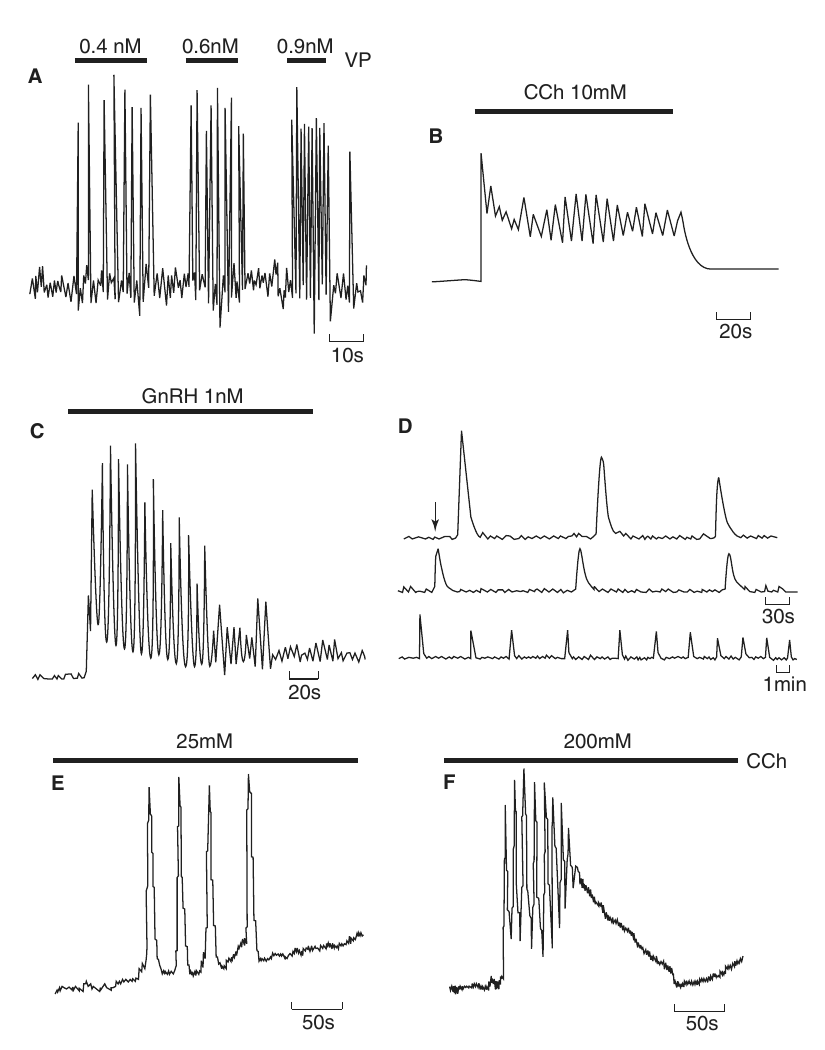
\includegraphics[width=.99\textwidth]{rysunki/rozdzial_2/differentoscilations.png}
\caption[Rodzaje oscylacji wapniowych]{Rożne rodzaje oscylacji jonów wapnia w wielu typach komórek eukariotycznych. A: hepatocyty stymulowane wazopresyną; B: komórki ślinianek aktywowane karbacholem (CCh)\nomenclature{CCh}{karbachol}; C: komórki gonadotropowe tylnego płata przysadki mózgowej stymulowane gonadoliberyną (GnRH)\nomenclature{GnRH}{gonadoliberyna}; D: oocyty chomika tuż po zapłodnieniu; E, F: komórki nowotworowe wywodzące się z limfocytów typu B, stymulowane dwoma różnymi stężeniami karbacholu \cite{Keener2009}, str. 277.}
\label{fig:oscylacje}
\end{figure}


Wzbudzenie oscylacji wapniowych w komórce oparte jest na mechanizmie ,,wszystko albo nic'', tzn. pojawiają się dopiero po osiągnięciu pewnego progu pobudzenia. Dalszy wzrost stymulacji może prowadzić do zwiększenia częstotliwości oscylacji, ale nie ma wpływu na amplitudę \cite{Keener2009}.

W ciągu ostatnich 30 lat powstało wiele modeli matematycznych, które wyjaśniały powstawanie i charakter oscylacji wapniowych.  Modele te różniły się pod względem precyzji opisu i~zależne były od szeregu założeń, które leżały u podstaw konstrukcji danego modelu. Opisywały oscylacje wapniowe z różnej perspektywy. Uproszczona klasyfikacja modeli przestawiona została wraz z przykładami w Tablicy~\ref{tab:modele} \cite{Dupont2011}.

Schemat przepływów jonów wapnia w modelu dwu-kompartmentowym (two-pool), ograniczający się do przepływów pomiędzy retikulum endoplazmatycznym a cytozolem oraz wymianę ze środowiskiem zewnątrzkomórkowym przedstawiony został na Ryc.~\ref{fig:sneydschemat}. Przyjmując, że ilość jonów wapnia jest stała w układzie, schemat ten można przedstawić za pomocą równań:

\begin{eqnarray}
\frac{dc}{dt} &=& J_{ch} -J_{pump} + J_{in} - J_{PMCA}\\
\frac{dc_{ER}}{dt} &=& \gamma(J_{pump} - J_{ch})
\end{eqnarray}

\noindent W równaniach tych $c$ oznacza stężenie jonów wapnia w cytozolu uśrednione po jego objętości. $c_{ER}$ oznacza natomiast stężenie jonów wapnia w retikulum endoplazmatycznym. $\gamma$ to stosunek objętości cytozolu do objętości kompartmentu:

\begin{equation}
\gamma = \frac{V_{Cyt}}{V_{ER}}
\end{equation}

$J_{ch}$ to wypływ jonów wapnia przez kanały wapniowe z ER do cytozolu, $J_{pump}$ napływ jonów wapnia do ER z cytozolu, oraz analogiczne prądy wapniowe realizowane przez kanały i pompy wapniowe na powierzchni błony komórkowej ($J_{in}$ wpływ jonów Ca$^{2+}$ do cytozolu, $J_{PMCA}$ usuwanie jonów Ca$^{2+}$ z cytozolu do przestrzeni zewnątrzkomórkowej).  Takie modele nazywane są \textbf{modelami otwartymi}, gdyż wapń może przepływać pomiędzy przestrzenią zewnątrzkomórkowa, a cytozolem \cite{Keener2009,Sneyd2004}. Oscylacje wynikające z powyższego modelu widoczne są na Ryc.~\ref{fig:sneydoscylacje}.

\begin{wrapfigure}{o}{0.5\textwidth}
	%\vspace{25pt}
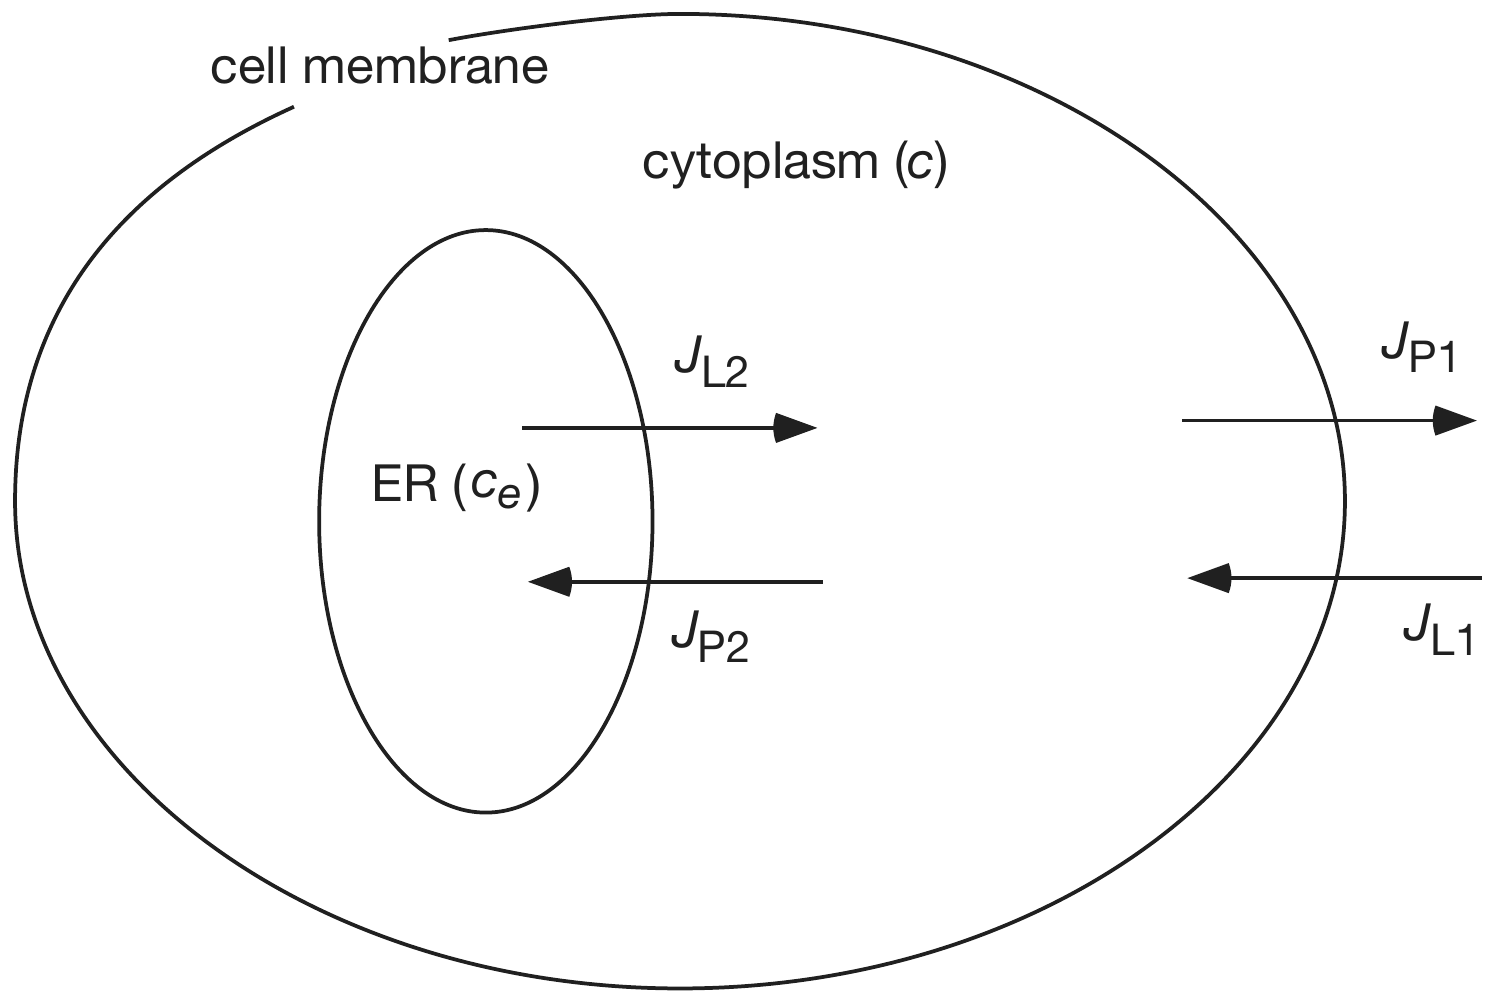
\includegraphics[width=0.5\textwidth]{rysunki/rozdzial_2/sneydSchematic.png}
\caption[Diagram prostych oscylacji]{Diagram przedstawiający typowe przepływy jonów wapnia w prostym modelu CICR w~neuronach żaby ryczącej \cite{Keener2009}.}
\label{fig:sneydschemat}
\end{wrapfigure}

W niektórych modelach zakłada się, ze względu na niewielką wymianę jonów Ca$^{2+}$ ze środowiskiem zewnętrznym, że ilość jonów wapnia w komórce pozostaje stała:

\begin{equation}
\gamma c + c_{ER} = constans
\end{equation}

\noindent Takie modele nazywają się \textbf{modelami zamkniętymi} \cite{Keener2009}.

Zauważmy, że przedstawiony powyżej model dwu-kompartmentowy jest często redukowany do modelu jedno-kompartmentowego, w którym rozważa się jedynie stężenie wolnych jonów wapnia w cytozolu, a przepływy jonów wapnia pomiędzy cytozolem a~retikulum realizowany jest poprzez dodanie odpowiedniej funkcji źródłowej. Z drugiej strony możliwe jest rozszerzenie modelu na dodatkowe kompartmenty (np. mitochondria \cite{Marhl2000}, jądro komórkowe \cite{Alonso2006} oraz uwzględnienie dodatkowych zjawisk np. przemian zachodzących na powierzchni błony komórkowej \cite{Hernjak2005}). Można również uwzględnić obecność białek buforujących w każdym z kompartmentów poprzez wprowadzenie odpowiedniej stałej skalującej przed przepływami z danego kompartmentu \cite{Marhl2000}. W przypadku modeli przestrzennych obecność buforów uwzględnia się poprzez  modyfikację funkcji źródłowych, jak również poprzez wprowadzenie efektywnego współczynnika dyfuzji wapnia (istotnie mniejszego od średnicy komórki).

\begin{wrapfigure}{o}{0.5\textwidth}
	%\hspace{25pt}
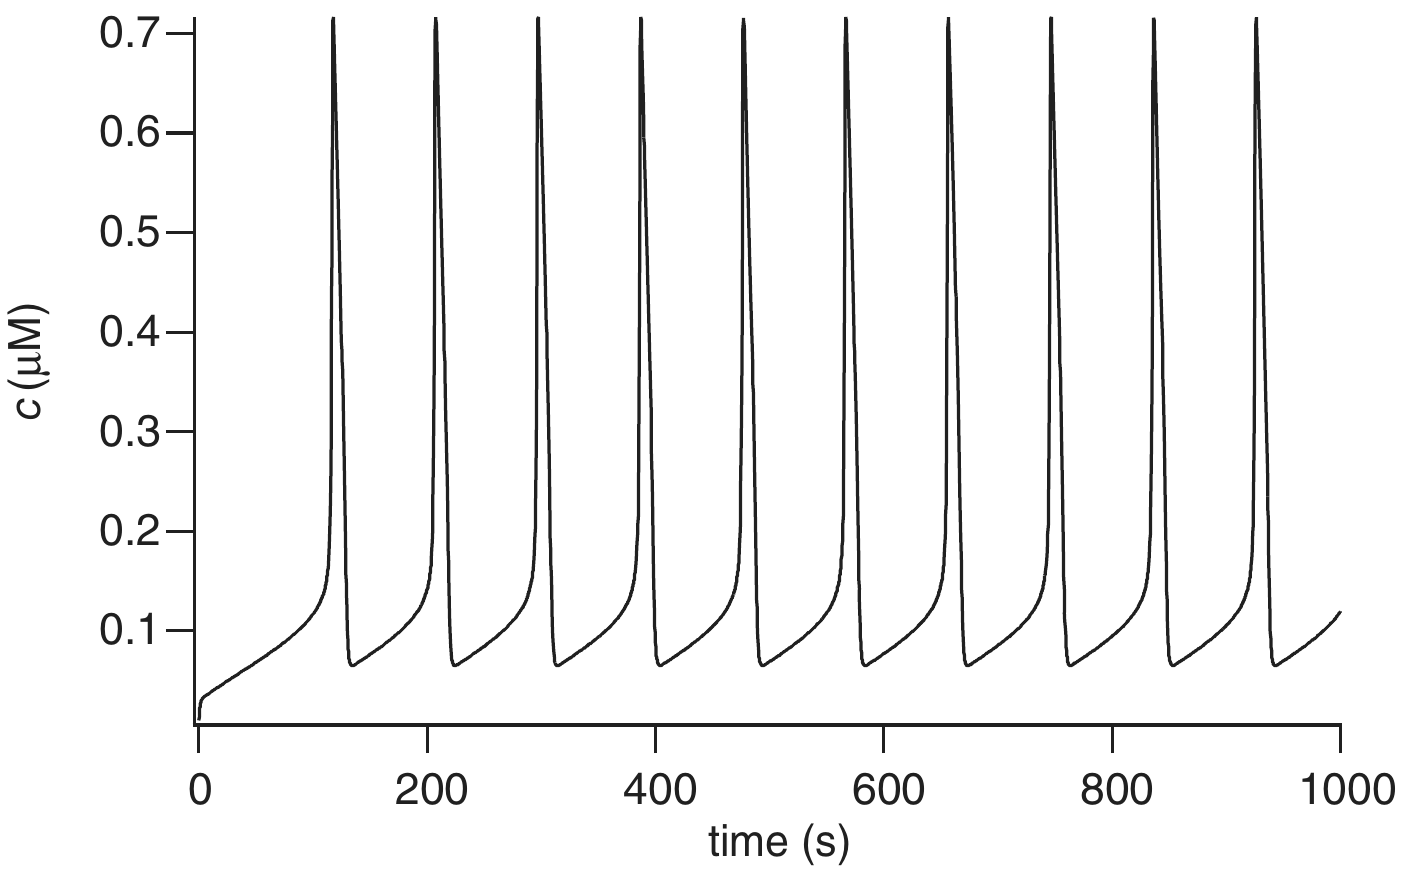
\includegraphics[width=0.5\textwidth]{rysunki/rozdzial_2/sneydoscilations.png}
\caption[Oscylacje wapniowe w modelu Sneyda]{Typowe oscylacje reprodukowane w modelu prostych oscylacji jonów wapnia. Dla $c_0$ = 1000 µM~\cite{Keener2009}.}
\label{fig:sneydoscylacje}
\end{wrapfigure}

W wielu przypadkach oscylacje wapniowe nie są zjawiskiem regularnym, lecz pojawiają się w sposób chaotyczny i posiadają stochastyczny charakter \cite{Falcke2004}. Spowodowane to jest stochastyczną naturą zjawiska otwierania i zamykania się kanałów wapniowych (np.IP$_3$R/RyR). Może się zdarzyć, że w wiele obserwowanych oscylacji, mimo swojej regularności powstała w wyniku procesów  stochastyczny, a~nie deterministycznych mechanizmów oscylacyjnych.

\bigskip

\begin{small}
\begin{longtable}{llP{9cm}r}
\caption[Uproszczona klasyfikacja modeli oscylacji wapniowych]{Uproszczona klasyfikacja modeli oscylacji wapniowych - przekrój.}\label{tab:modele}\\
	\toprule[0.12em]
	\textbf{Autor}    & \textbf{Rok}  & \textbf{Opis}      &      \textbf{Referencje} \\\midrule[0.06em]
	\endfirsthead
	\multicolumn{4}{c}%
	{\tablename\ \thetable\ -- \textit{Uproszczona klasyfikacja modeli oscylacji wapniowych - kontynuacja\ldots}} \\
	\toprule[0.17em]
	\textbf{Autor}    & \textbf{Rok}  & \textbf{Opis}      &      \textbf{Referencje} \\\midrule[0.1em]
	\endhead
 \multicolumn{4}{r}{\textit{Kontynuacja na następnej stronie\ldots}} \\
	\endfoot
	\endlastfoot
\ngray \multicolumn{4}{c}{\textbf{Deterministyczne}}\rule[-2ex]{0pt}{5.5ex}  \\
Mayer         & 1988 & Model oscylacji indukowanych receptorem na powierzchni komórki & \cite{Meyer1988}\\
Goldbeter     & 1990 & Zamknięty, mechanizm CICR         & \cite{Goldbeter1990} \\
Semogyi       & 1990 & Otwarty, oscylacje wapnia w hepatocytach, uwzględniał regulator białkowy - kalmodulinę & \cite{Somogyi1991} \\
DeYong        & 1992 & Ośmiostanowy model receptora IP$_3$ & \cite{DeYoung1992} \\
Atri          & 1993 & Jednokompartmentowy, opisuje oscylacje Ca$^{2+}$ w~cytozolu oocytu & \cite{Atri1993} \\
Tang          & 1994 & Model oscylacji w miocytach & \cite{Tang1994}\\
Keizer        & 1996 & Model kanału RyR                  & \cite{Keizer1996} \\
Borghans      & 1997 & Otwarty, 2kompartmenty            & \cite{Borghans1997} \\

Marhl         & 2000 & Trzy kompartmenty: Ca, ER, Mit    & \cite{Marhl2000} \\
Bindschadler  & 2001 & Międzykomórkowy, 2 kompartmenty   & \cite{Bindschadler2001} \\
Sneyd         & 2002 & Model kanału IP$_3$R              & \cite{Sneyd2002} \\
Fridlyand     & 2003 & Zamknięty 2 kompartmenty, oscylacje wapnia w~komórkach trzustki   & \cite{Fridlyand2003} \\
Oxhamre       & 2005 & Zamknięty, 2 kompartmenty, oscylacje indukowane infekcją bakteryjną  & \cite{Oxhamre2005} \\
Wang          & 2007 & Oscylacje wapniowe wzbudzone ATP & \cite{Wang2007} \\
Dash          & 2008 & Model wymienników mitochondrialnych  & \cite{Dash2008}\\
Dash          & 2009 & ,,Mechanistyczny'' model uniportera mitochondrialnego, który uwzględnia rolę potencjału transbłonowego i~zmiany konformacji uniportera & \cite{Dash2009}\\
Zeng          & 2009 & Spontanicznie indukowane oscylacje wapniowe w~astrocytach & \cite{Zeng2009}\\
Dyzma         & 2012 & Trój-kompartmentowy model uwzględniający mikrodomeny ER-Mit & \cite{Dyzma2012}\\
\ngray \multicolumn{4}{c}{\textbf{Stochastyczne}}  \rule[-2ex]{0pt}{5.5ex}  \\
Magnus        & 1998 & Model oscylacji Ca$^{2+}$ w komórkach trzustki ($\beta$) z~uwzględnieniem właściwości elektrycznych komórek (transport pozostałych jonów) & \cite{Magnus1998a,Magnus1998}\\
Coombes       & 2004 & Model "iskier" powstających podczas otwierania się kanałów wapniowych w magazynach komórkowych & \cite{Coombes2004} \\
Kummer        & 2005 & Porównanie modelu stochastycznego w stosunku do modeli deterministycznych & \cite{Kummer2005} \\
Keener        & 2006 & & \cite{Keener2006}\\
Dupont        & 2008 & Model oscylacji wapniowych w hepatocytach & \cite{Dupont2008} \\
\ngray \multicolumn{4}{c}{\textbf{Mieszane}}\rule[-2ex]{0pt}{5.5ex} \\
Bazil         & 2011 & Model mechanizmu RaM & \cite{Bazil2011} \\
\ngray \multicolumn{4}{c}{\textbf{Przestrzenne}}\rule[-2ex]{0pt}{5.5ex} \\
Wagner        & 1994 & Rola szybkich buforów w modelach dyfuzji i oscylacji jonów wpania& \cite{Wagner1994} \\
Dawson        & 1999 & Model fal wapniowych w postaci serii pulsów wapniowych wzdłuż ER & \cite{Dawson1999}\\
Falcke        & 2000 & Fale spiralne w oocycie & \cite{Falcke2000} \\
Fink          & 2000 & Fale wapniowe wywołane bradykininą w komórkach neuroblastomy, geometria bazująca na zdjęciach mikroskopowych komórek & \cite{Fink2000} \\
Falcke        & 2003 & Stochastyczny, przestrzenny & \cite{Falcke2003} \\
Falcke        & 2003 & Model dyfuzji buforów wapniowych & \cite{Falcke2003a}\\
Higgins       & 2007 & Model mikrodomen pomiędzy sarkomerami w~kardiomiocycie & \cite{Higgins2007}\\
Thul          & 2008 & Model dyfuzji seryjnych wyładowań jonów wapnia z~magazynów ER w postaci fal & \cite{Thul2008a}\\
Kaźmierczak   & 2010 & Fale biegnące w komórkach o zróżnicowanej geometrii & \cite{Kazmierczak2010} \\
 \bottomrule[0.12em]
\end{longtable}
\end{small}